In the last years, 2D materials with interesting properties were synthesized.\textcolor{red}{\textbf{citation}} One of it is hexagonal boron nitride (\textit{h}-BN).\textcolor{red}{\textbf{citation}} It is made up of the same number of nitrogen and boron atoms. They are arranged in an $\textnormal{sp}^2$-bonded honeycomb lattice so that each nitrogen is neighbored by boron atoms and vice versa. The ionic bond character between both is a direct result from the nitrogens larger electrochemical negativity, withdrawing electrons from the boron lattice site and making \textit{h}-BN an insulator with wide band gap of approximately \SI{6}{\eV}. \cite{watanabe_direct-bandgap_2004, cassabois_hexagonal_2016, blase_quasiparticle_1995}

Free standing \textit{h}-BN is investigated with \textit{ab-initio} calculations \cite{han_effects_2014,mortazavi_investigation_2012,topsakal_first-principles_2009,peng_mechanical_2012}. Together with experiments \cite{paszkowicz_lattice_2002} a crystal lattice constant of $a_{\textit{h}-BN, RT}=\SI{2.504}{\angstrom}$ is derived. 

It can be grown on a variety of metal surfaces.\textcolor{red}{\textbf{citation}} Depending on the substrates used, different lattice mismatches can be achieved. Many geometric corrugations can be achieved with increasing lattice mismatch and substrate-\textit{h}-BN interaction. Since this interaction is believed to have its origin in the partially filled d-states of the substrate,\textcolor{red}{\textbf{citation}} transition metal substrates are widely used. While substrates exist where the lattice constant are virtually identical (Ni: $\Delta \leq \SI{0.5}{\percent}$), other substrates like Ag(111) show large mismatches ($\Delta \approx \SI{14}{\percent}$). 

The growth of \textit{h}-BN on nearly lattice matched Ni(111) resulted in uniform commensurate layers. With increasing lattice mismatch, moir\'e patterns are formed on Pd and Pt. The stronger interaction of \textit{h}-BN and Rh(111) results in a corrugated nanomesh to be formed on the substrate.\textcolor{red}{\textbf{citation}} Even 1D structures are reported on Fe(110) \cite{vinogradov_one-dimensional_2012} and Cr(110) \cite{muller_one-dimensional_2008}. 

Here we consider \textit{h}-BN on Cu(111) as example system of self-limited growth and highlight most relevant insights reported in literature.\cite{joshi_boron_2012, schwarz_corrugation_2017, auwarter_hexagonal_2018}

\subsubsection{on Cu(111)}
%\begin{table}\centering
%	\caption{Lattice mismatches between \textit{h}-BN and several transition metal surfaces. The mismatch is given to describe the relative size of the \textit{h}-BN layer compared to the substrate, e.g. negative values indicate a larger lattice constant in the substrate bulk. Information adopted from \cite{_ptable}}
%	
%	\begin{tabular}{cccl}
%		Substrate 	& Mismatch [\%] 		& Electronic configuration \\ \hline
%		Ni(111)		& \SI{+0.4}{\percent} 	& [Ar] 3d8 4s2	\\
%		Cu(\left( 111)		& \SI{-1.9}{\percent} 	& [Ar] 3d10 4s1	\\	
%		 \\
%	\end{tabular}
%	\label{tab:h-BN-mismatch}
%\end{table}

	\paragraph{Stoichiometry}
	XPS measurements (see \autoref{fig:XPS-hbn-Cu111-martin}) show B\textit{1s} and N\textit{1s} components in a 1:1 ratio, indicating that the layer retains the precursor stoichiometry during growth, but all hydrogens are cleaved from the precursor prior to layer formation and desorp from the sample.\cite{Zhang_Two-dimensional_2017}
	
\begin{figure} \centering
	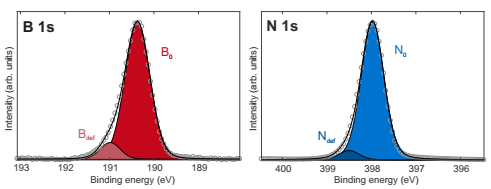
\includegraphics[width=0.7\textwidth]{./images/XPS-hbn-Cu111-martin}%
	\caption{XPS of a full ML \textit{h}-BN on Cu(111) grown with CVD. Fit components $B_0$ ($E_b=\SI{190.4}{\eV}$), $N_0$ ($E_b=\SI{398.0}{\eV}$) and $B_{def}$ ($E_b=\SI{191.0}{\eV}$) and $N_{def}$ ($E_b=\SI{398.5}{\eV}$) are assigned to pristine \textit{h}-BN layer and defective components respectively. Adopted from \cite{schwarz_assembly_2018}}
	\label{fig:XPS-hbn-Cu111-martin}
\end{figure}



	\paragraph{Moir\'e geometry}
	The properties of various moir\'e superstructures are well described in literature and Hermann gives a comprehensive overview in his paper.\cite{hermann_periodic_2012}\label{section:moire}
	
	If lattice constants are equal like in the case of a graphene bilayer, the needed lattice mismatch occurs due to a rotation of the two layers. A moir\'e is always present if an over layer shows a lattice mismatch with respect to the substrate. 
	
	For \textbf{isotropically scaled over layers} one can calculate the scaling factor $$p=\frac{R^{'}_{O1}}{R_{O1}}$$ which gives the size of the over layer lattice $R^{'}_{O1}$ in units of the substrate lattice $R_{O1}$. The moir\'e pattern shows the same bravais lattice type than the substrate\cite[10]{hermann_periodic_2012}. If moir\'e and ad layer lattice are aligned ($\alpha=0$\textdegree) the direction of moir\'e and substrate is aligned. If the over layer is isotropically scaled and not rotated, the period of the moir\'e calculates to $$a_{moir\'e}=\underbrace{\frac{p}{|p-1|}}_{\kappa}a_{substrate}$$
	With $a_{moir\'e}$ and $a_{substrate}$ are experimentally available, the ad layer lattice can be calculated with high precision (usually one order of magnitude more accurate than direction measurement of its period).\cite{farwick_zum_hagen_structure_2016}

Depending on the relative orientation of \textit{h}-BN and substrate the moir\'e period changes. Although large domains with uniform orientation can be grown on single crystal substrates (\autoref{fig:moire-STM-model}(a,c)), rotational domains exist(\autoref{fig:moire-STM-model}(b,d,e)).
The model representation nicely shows the change in moir\'e period when
\autoref{fig:moire-STM-model}(c) shows a case where the \textit{h}-BN ad layer has the same unit cell orientation than the copper. For a \textbf{scaled and rotated over layer} the angle between substrate and moir\'e ($\gamma$[rad]) scales with the angle between over layer and substrate ($\alpha$[rad]) as $\alpha=(1-p)\gamma$.
For rotated and isotropically scaled over layers, one can determine the $\alpha$ and $p$ from experimental observables $\gamma$(moir\'e angle to substrate) and $\kappa$(scaling factor) through relations $ \alpha=\arctan \left ( \frac{sin(\gamma)}{cos(\gamma)+\kappa} \right )\qquad p=\frac{\kappa}{\sqrt{1+\kappa^2+2\kappa cos(\gamma)}}$

\begin{figure} \centering
	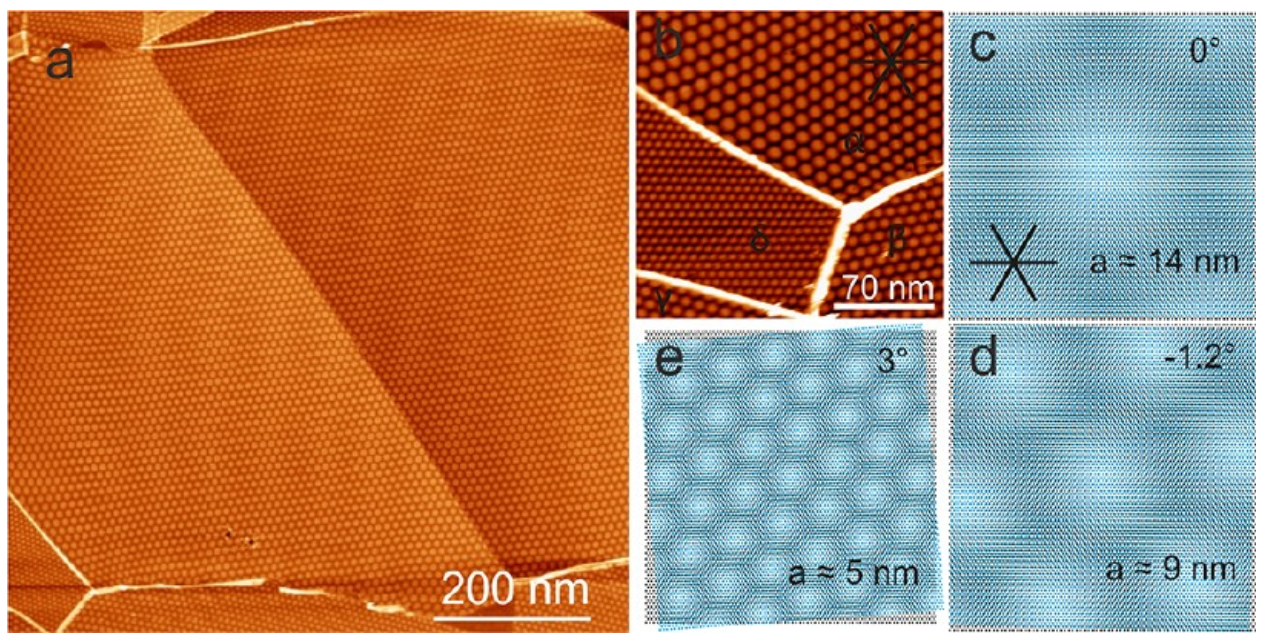
\includegraphics[width=0.5\textwidth]{./images/h-BN-cvd-cu111.png}%
\caption{(a) STM topography of \textit{h}-BN on Cu(111). Large domains with uniform orientation and moir\'e period are formed after CVD growth. (b) Different rotational domains are observed that show different moir\'e periods, reproduced by three models (c-e) where different \textit{h}-BN rotations are shown together with the resulting moir\'e periods a. Adopted from \cite{joshi_boron_2012}}
\label{fig:moire-STM-model}
\end{figure}

As mentioned above the orientation of the moir\'e superstructure is determined by the relative ad layer rotation alone, while its period is determined by lattice mismatch, too. This results in a variety of moir\'e superstructure orientations and periods, strongly related to the used substrate.
	
\paragraph{Periodic change in work function}
A direct result of the lattice mismatch between \textit{h}-BN and substrate is the alternating registry of ad layer atoms and substrate. The periodic modulation of B/N registry to the substrate atoms results in regions of stronger and weaker interaction between \textit{h}-BN and substrate and is the reason for the nano templating effect of \textit{h}-BN on many substrates.\textcolor{red}{\textbf{citation}} In the following some effects are discussed that lay the foundation for a nano patterning effect of \textit{h}-BN and its influence on the electronic structure of adsorbates.

While a first report in 2004 \cite{corso_boron_2004}, pointed to the formation of a complicated two layer structure, later experiments \cite{roth_chemical_2013, li_grain_2015} including ours \cite{joshi_boron_2012, schwarz_corrugation_2017} and others \textit{h}-BN/Cu(111) proofed a single layer of B \& N atoms in a regular hexagonal lattice. It evolved as well investigated system to perform experiments on. It could be shown that after CVD growth it adsorbs on Cu(111) as a flat layer. Due to its  lattice mismatch, "hill" regions  (corresponding to a $N_{top}B_{fcc}$ registry) and "valleys" (corresponding to a $N_{fcc}B_{hcp}$ registry) are formed. In these regions the work function is altered in opposite directions. While larger at the hill/pore regions, the work function reduces continuously to its lowest value in the valley/wire regions.\footnote{Please note that the notation is not uniform throughout the literature. Sometimes hills are referred to as pores and valley regions are denoted as wire regions.} 

Everywhere two regions with different work functions meet, \textbf{local electrostatic fields} arise to compensate for the vacuum level misalignment.

After growth of \textit{h}-BN the substrates over all work function is reduced [e.g. Rh: \SIrange{5.01}{3.07}{\eV} \cite{gomez_diaz_hexagonal_2013}. Therefor a dipole moment $\mu$ pointing from the the bulk to the surface is necessary, rather likely created by a negative charge transfer from the bulk into the ad layer.\cite{roman_periodic_2013}


\begin{figure} \centering
	\subfigure[Work function variation along \textit{h}-BN/Cu(111) moir\'e. (a) STM image showing the \textit{h}-BN moir\'e with a periodicity of 8.4 nm. Scan parameter: $U_b= 4.0 V, I_t= 40 pA$. (b)	Field emission resonances acquired along the black dotted line in a) revealing a variation of the peak positions. (c) Work  function  differences  between bright  (“hill”/pore)  and  dark  (“valley”/wire)  regions obtained  from  the  dI/dV curves  of  the  field emission  resonances  displayed  in  b). Adopted from \cite{schwarz_corrugation_2017}]{
		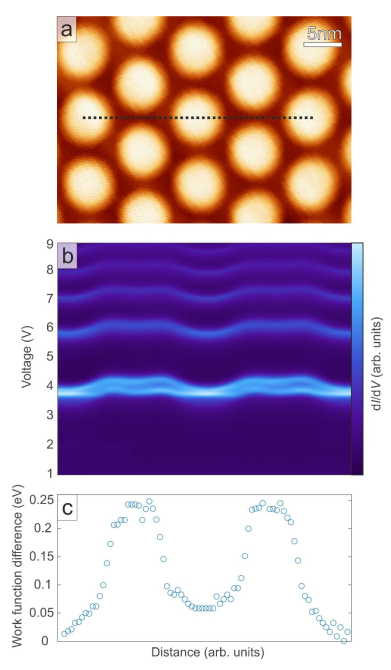
\includegraphics[width=5cm]{./images/h-BN-Cu(111)-wf-change}
	\label{fig:h-BN-Cu(111)-wf-change-I}
		} \quad
	\subfigure[Position dependent energy level alignment of $NC-Ph_4-CN$ on \textit{h}-BN/Cu(111). Three spectra are compared, recorded on molecules at valley (blue) and hill positions (green). A spectrum of the bare Ag(111) is shown as reference. Taken from \cite{diss-joshi}]{
	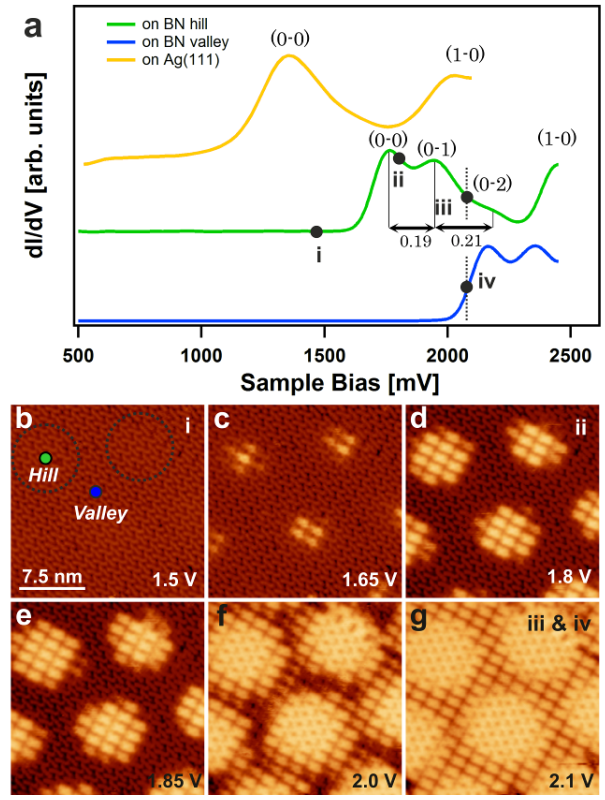
\includegraphics[width=6cm]{./images/h-BN-Cu(111)-wf-change-II}
	\label{fig:h-BN-Cu(111)-wf-change-II}
	}
	\label{fig:h-BN-Cu(111)-wf-change}
\end{figure}

\paragraph{Molecular adsorption and assembly}
\label{section:Mol-on-h-BN}
\textcolor{red}{\textbf{Write some more - explain examples - how does the assembly process work?}}

With changing work function, a lateral electric field emerges. For gr/Ru(0001) lateral dipole pointing from valley to pore sites arise.\cite{zhang_assembly_2011} It can be used to trap adsorbates with dipole moment along the field lines. This was shown for FePc and pentacene molecules on a graphene/Ru(0001) substrate. Here FePc molecules adsorp first on regions with high lateral dipole along top-fcc direction (valley), followed by regions with lower lateral dipole (on the hill). Pentacene molecules are trapped along the top-fcc direction, too.\cite{zhang_assembly_2011}  This general adsorption mechanism is applicable for other systems with periodic modulation of the work function.

\autoref{fig:h-BN-Cu(111)-wf-change} depicts the work function change measured with STS (Field emission resonances) indicating a similar modulation of the work function. In this theses TBP molecules (\autoref{section:TBP}) and helicene molecules (\autoref{section:helicene}) are used as sample molecules for specific adsorption site or orientation alignment.

It was shown that this moir\'e superstructure influences molecular assembly. 
\textcolor{red}{\textbf{Explain the Porphine adsorption on metal and on \textit{h}-BN}}

\begin{figure} \centering
	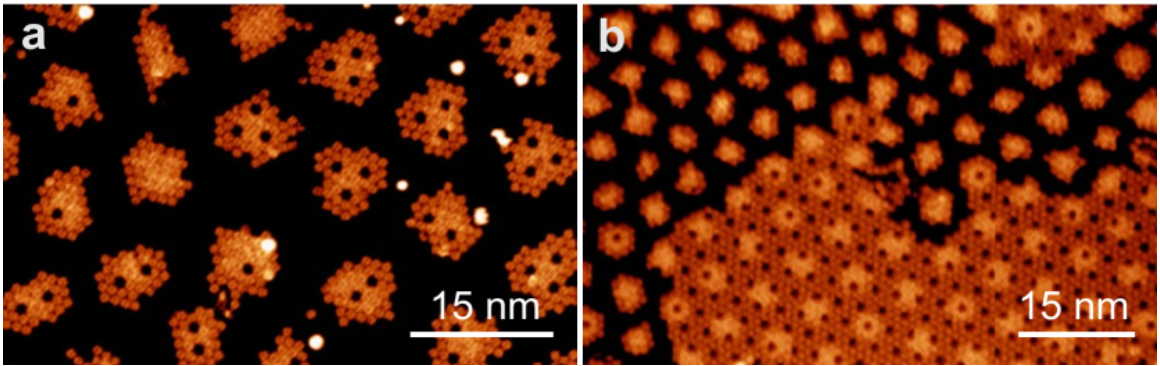
\includegraphics[width=0.7\textwidth]{./images/2H-P-hBN-Cu111-joshi}%
	\caption{STM topography of 2H-P adsorped on \textit{h}-BN/Cu(111). (a) A large moir\'e domain guides the formation of small 2H-P islands with off center vacancies. (b) High coverage overcomes the template effect of the \textit{h}-BN support. Adopted from \cite{diss-joshi}}
	\label{fig:2H-P-hBN-Cu111-joshi}
\end{figure}

\textbf{Molecules are electronically decoupled} when adsorped on a \textit{h}-BN spacer layer on top of a metal. The insulating \textit{h}-BN hinders the metal to influence molecular properties by charge transfer, image potentials etc.\textcolor{red}{\textbf{citation}}. As a result, molecular orbitals are unperturbed and can be imaged in STM/STS.